%El presente capítulo describe el modelo de negocios para el módulo de Registro de escuelas, el cual es utilizado dentro del desarrollo del {\bf \varProyecto}, el cual se conforma de los siguientes elementos:

El presente capítulo describe el modelo de negocios correspondiente al TLAMATINIME: Timetabling Problem, Prototipo de Optimización de Horarios
en la ESCOM, el cual se conforma de los siguientes elementos:

\begin{itemize}
    \item Modelo de información. En esta sección se presentan los atributos y relaciones de toda la información que contemplará el sistema en los módulos de Academias, Infraestructura, Oferta Educativa, Profesores y Estructura Educativa. \\
    
    En la figura~\ref{fig:modeloER} se muestra el Modelo Entidad Relación del sistema.
    
    \begin{figure}[htbp!]
    	\begin{center}
    		\fbox{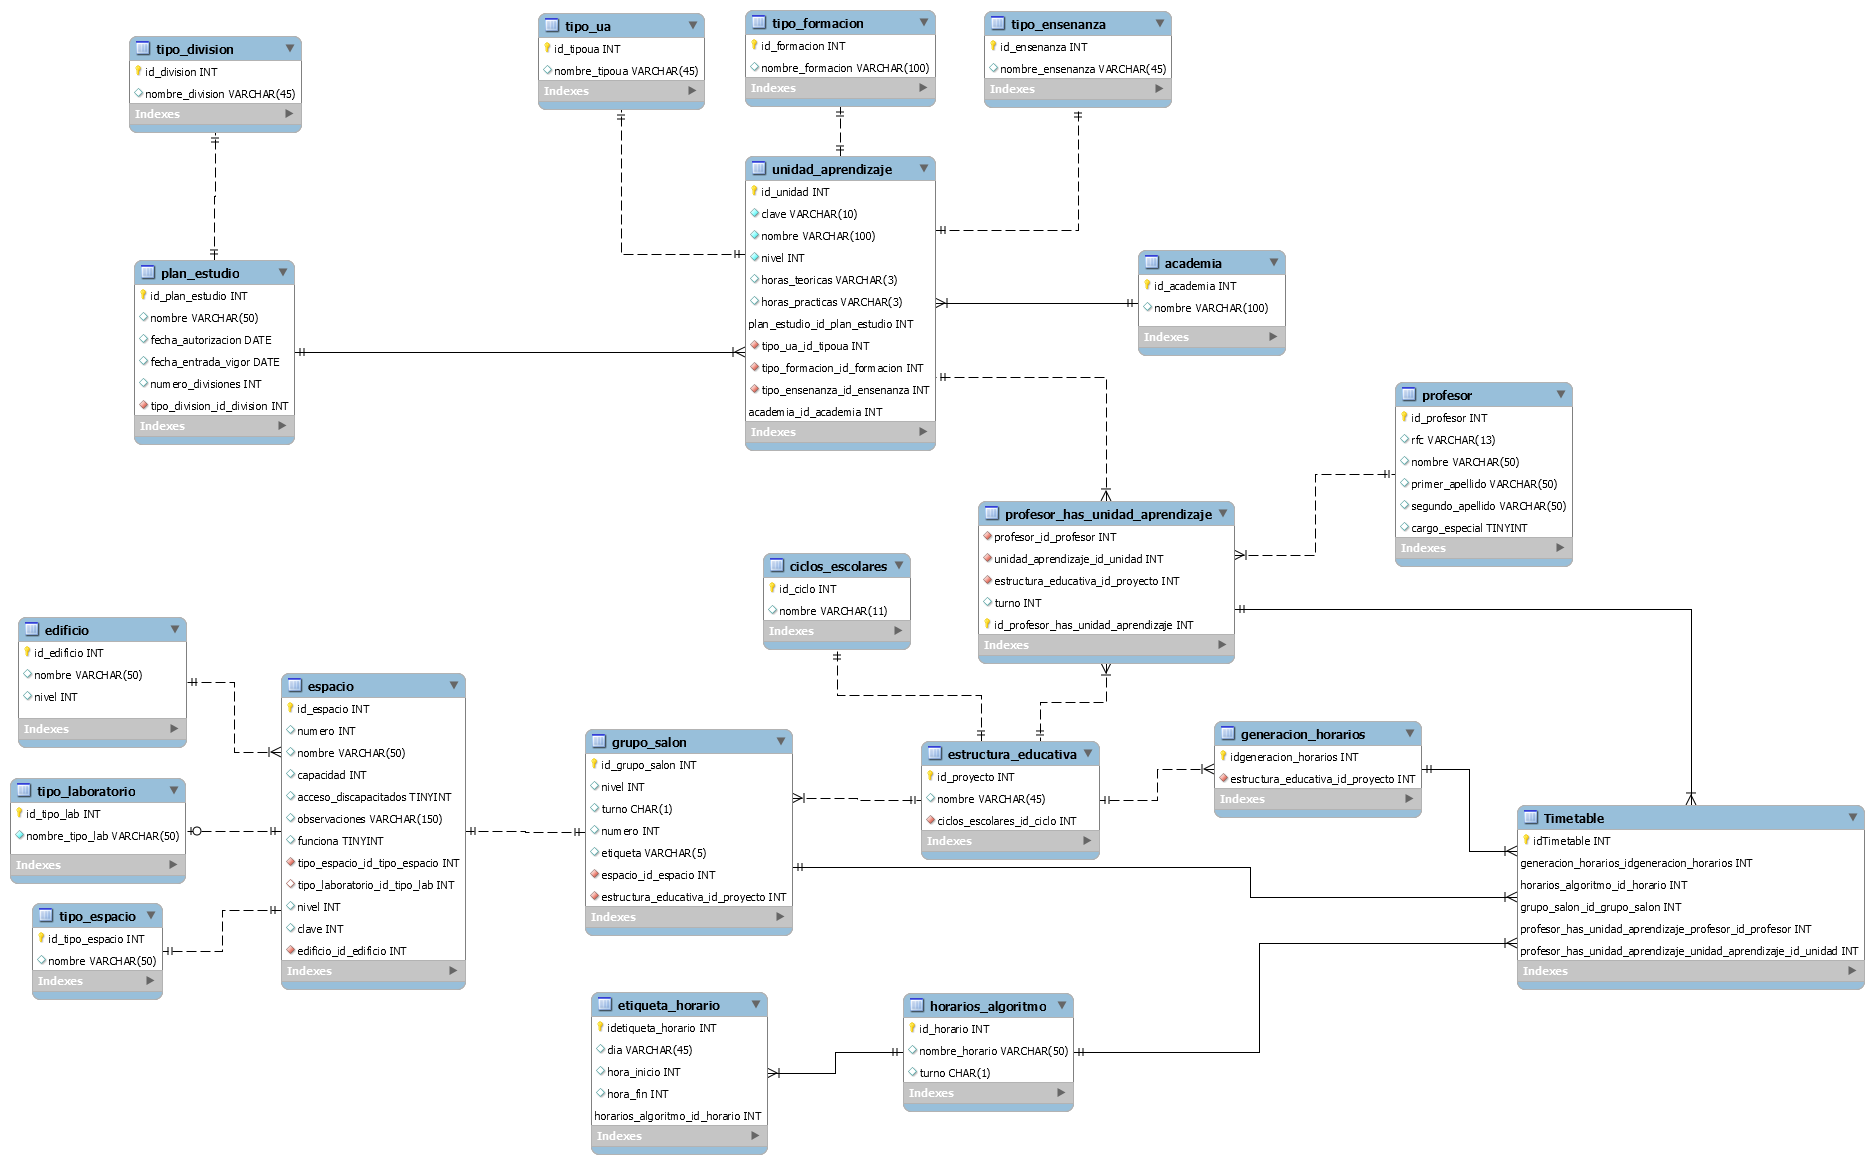
\includegraphics[width=1\textwidth]{images/entornoTT/modeloER.png}}
    		\caption{Modelo Entidad Relación del sistema.}
    		\label{fig:modeloER}
    	\end{center}
    \end{figure}

    % Registro de escuelas, Información base para indicadores, Plan de acción, Seguimiento y acreditación e Indicadores.

    \item Reglas de negocio. Son las directivas destinadas a gobernar, guiar o influenciar el comportamiento de los procesos de negocio.
     %Son las directivas que expresan una política de negocio, es decir, describen, limitan o controlan un determinado aspecto del negocio.\\
\end{itemize}

